\chapter{Method}

% \section{Voxelnet}
% VoxelNet is an End-to-End Learning for Point Cloud Based 3D Object Detection. The work is described in Yin Zhou and Oncel Tuzel's paper: \cite{https://doi.org/10.48550/arxiv.1711.06396}.

% In order to implement this work, the following git repo is adapted: \url{https://github.com/qianguih/voxelnet}. This repo contains a pre-trained model, trained to detect cars from the velodyne lidar data provided by the KITTI dataset.

% \section{ViperX 300 Robot Arm}
% In order to operate the Trossen Robotics ViperX 300 Robotic Arm, Their ROS 2 packages are utilised.
% These can be found here: \url{https://docs.trossenrobotics.com/interbotix_xsarms_docs/}.

This chapter will describe different methodologies used to solve technical problems over the course of this project.

\section{Problem Formulation}

The objective of this project is to set up an autonomous warehouse system where an autonomous UGV should be able to fetch objects in a warehouse. The system will rely on an UGV equipped for autonomous navigation to move around in the environment. The UGV will also be equipped with a robotic manipulator for pick and place operations.

\section{Hardware Setup}
The hardware setup of the system is determined by the tasks that the UGV should preform. The main functionality of the system can be divided into two main subsystems: an autonomously navigating UGV and a robot manipulator for pick-and-place operations. The "Husky A200" by Clearpath is chosen as a the UGV platform for the whole system. This is a ROS 2 compatible UGV with a rugged design that is suitable for both outdoor and indoor applications. The robotic manipulator of choice, is the "Interbotix VX300" by Trossen Robotics. This is a 12V powered compact manipulator that makes it easy to mount on the Husky UGV that has a 12V power distribution. Hardware overview is shown in figure \ref{fig:hardware_overview}.

\begin{figure}[H]
  \centering
  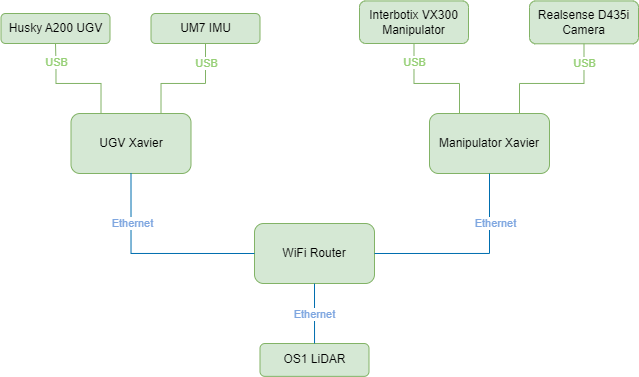
\includegraphics[width = 0.6\textwidth]{Figures/example_figure.drawio.png}
  \caption{Hardware overview of system}
  \label{fig:hardware_overview}
\end{figure}


\section{Software overview}
On a high level, the system is controlled by a ros node called "husky\_master". This node interacts with NAV2 and Moveit 2 to orchestrate an autonomous pick and place operation. The interaction between "husky\_master" and Moveit 2 is done through "husky\_pick\_and\_place" which acts as an interface between Moveit 2 and "husky\_master". A high level overview of this interaction is shown in figure \ref{fig:software_overview}

\begin{figure}[H]
  \centering
  \includegraphics[width = 0.6\textwidth]{Figures/software_overview.drawio.svg}
  \caption{Hardware overview of system}
  \label{fig:hardware_overview}
\end{figure}